\documentclass{article}
\usepackage[utf8]{inputenc} 
\usepackage[spanish]{babel}
\usepackage{url} 
\usepackage{enumerate}
\usepackage{graphicx}
\usepackage{float}
\usepackage{colortbl}
\usepackage[colorlinks=true,linkcolor=black,urlcolor=black, citecolor=black]{hyperref}

\begin{document}
\sloppy
\section*{Instalación de PrediXaber11}
\begin{enumerate}
\item Se debe tener instalado y configurado el JDK y el JRE version 7 de Java. En caso de no tenerlo, en \url{http://docs.oracle.com/javase/7/docs/webnotes/install/} se explica como instalarlo en distintos sistemas operativos.
\item Se debe tener instalado y configurado Apache Tomcat, en caso de no tenerlo, se pueden visitar las siguientes paginas, donde se indica como debe instalarse:
\begin{itemize}
\item Windows: \url{http://gonzasilve.wordpress.com/2013/04/13/instalacion-de-apache-tomcat-7-en-windows/}.
\item Linux: \url{http://nexolinux.com/apache-tomcat-7-instalacion/}.
\item Mac: \url{http://www.coconnut.com/blog/2012/03/15/instalar-apache-tomcat-en-mac-osx/}.
\end{itemize}
\item Cuando todo este correctamente instalado, debe ingresar al ``Manager App'' en Tomcat.
\begin{figure}[H]
\begin{centering}
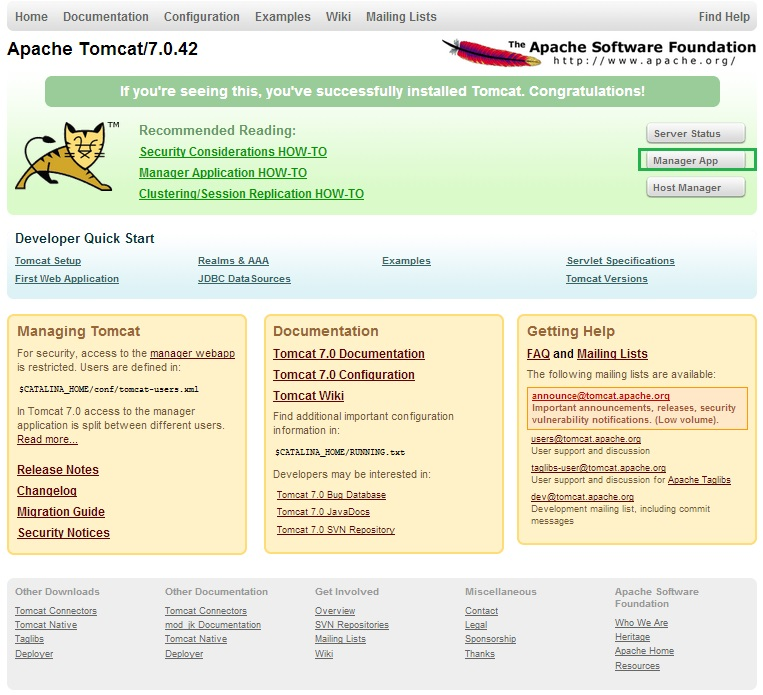
\includegraphics[scale=0.5]{tomcat6}
\par\end{centering}
\label{fig:figura6}
\end{figure}
\item En el panel ``Desplegar'' se debe seleccionar el archivo PrediXaber11.war y luego presionar en el boton ``Desplegar'' 
\begin{figure}[H]
\begin{centering}
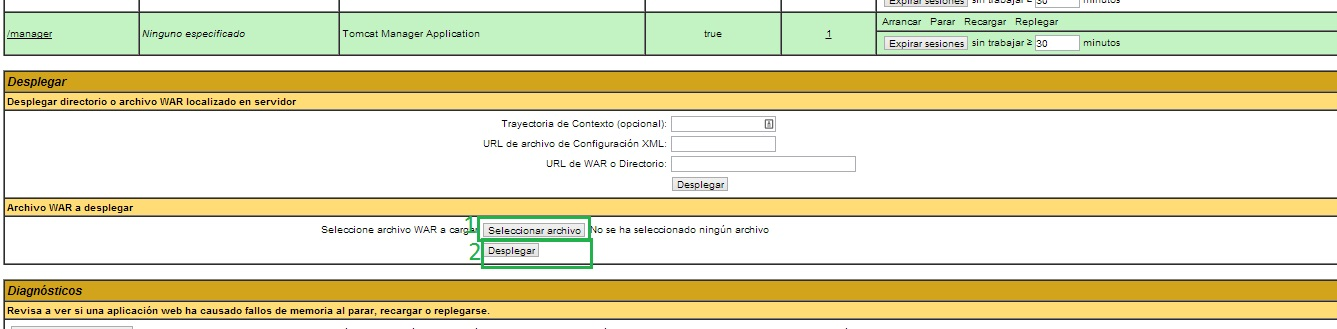
\includegraphics[width=12cm, height=5cm]{tomcat7}
\par\end{centering}
\label{fig:figura6}
\end{figure}
\item Despues de eso, en el panel ``Aplicaciones'' se encontrará /PrediXaber11.
\begin{figure}[H]
\begin{centering}
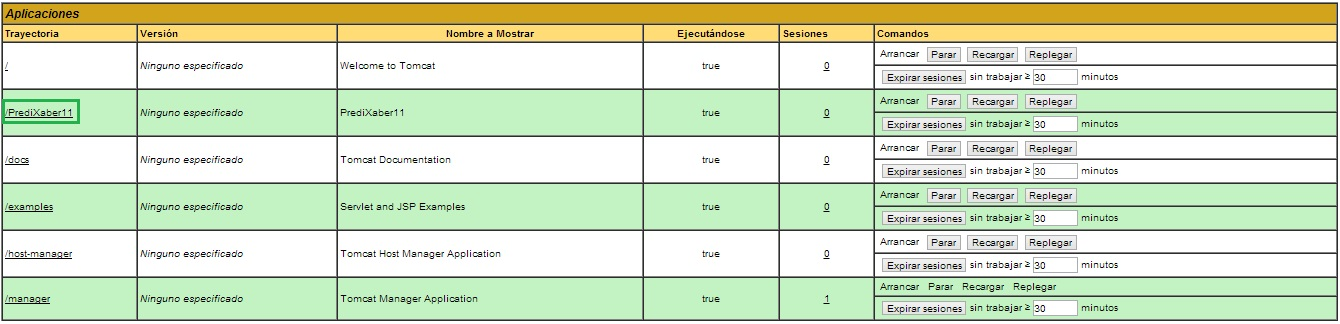
\includegraphics[width=12cm, height=5cm]{tomcat8}
\par\end{centering}
\label{fig:figura6}
\end{figure}
\item Presionar Click en el link y entonces se podrá interactuar con la aplicación PrediXaber11.
\begin{figure}[H]
\begin{centering}
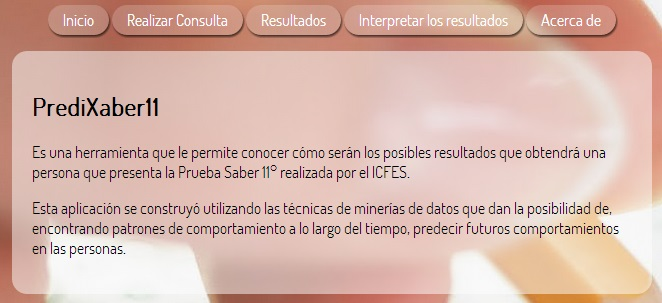
\includegraphics[width=12cm, height=5cm]{tomcat9}
\par\end{centering}
\label{fig:figura6}
\end{figure}
\end{enumerate}
\end{document}
